\documentclass[border=2px]{standalone}
\usepackage{graphicx}
\usepackage{tikz}

\usetikzlibrary{shapes.geometric, arrows}
\tikzset{
  box/.style = {draw, rectangle, minimum height=1.4cm, text width=3.0cm, text centered, draw=white, fill=white, font=\huge},
  to/.style  = {->, >=stealth', line width=2pt, draw=white, fill=white}
}


\begin{document}
\begin{tikzpicture}
    \node[anchor=south west,inner sep=0] (image) at (0,0,0) {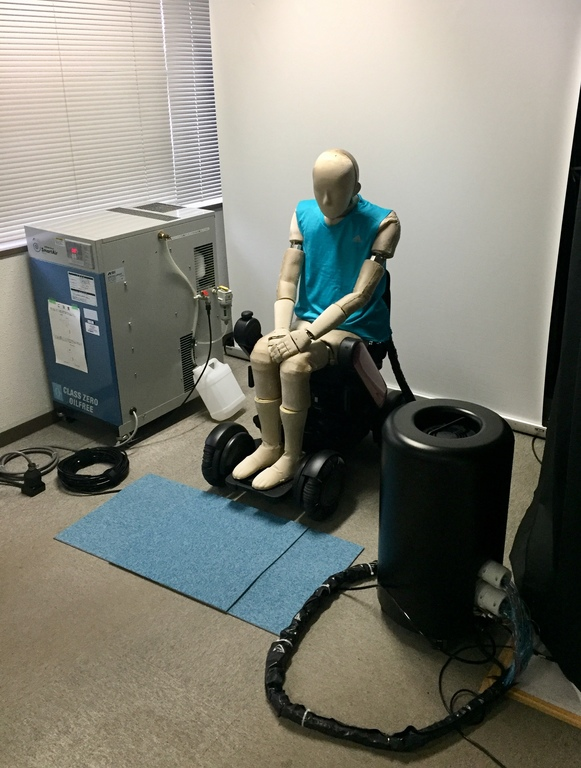
\includegraphics[width=\linewidth]{image}};
    \begin{scope}[x={(image.south east)},y={(image.north west)}]
        \iffalse
            % Next four lines helps to locate the point needed by forming a grid
            \draw[help lines,xstep=.1,ystep=.1] (0,0) grid (1,1);
            \draw[help lines,xstep=.05,ystep=.05] (0,0) grid (1,1);
            \foreach \x in {0,1,...,9} {\node[anchor=north] at (\x/10,0) {0.\x}; }
            \foreach \y in {0,1,...,9} {\node[anchor=east] at (0,\y/10) {0.\y};}
        \fi
        \begin{scope}[x={(image.south east)},y={(image.north west)}]
            %\draw[to] (0.85,0.70) node[box] {Whill (Electric Wheelchair)} -- (0.65,0.50);
            \draw[to] (0.10,0.40) node[box] {Air Compressor} -- (0.15,0.55);
            \draw[to] (0.40,0.25) node[box] {Robot Contoller} -- (0.65,0.25);
            \draw[to] (0.20,0.10) node[box] {Air Tubes} -- (0.45,0.10);
            \draw[to] (0.20,0.85) node[box] {Robotic Subject} -- (0.50,0.70);
        \end{scope}
    \end{scope}
\end{tikzpicture}
\end{document}
